\chapter{Introduction} \label{cap: Introduction}
\section{What is an Embedded Operating System?}
An \textbf{\textcolor{red}{operating system (OS)}} mediates \textbf{\textit{between application software and hardware}}. 
This \textbf{\textit{allows applications to request systems services, without needing to manually configure the hardware}}, like initialize the CPU, program timers, or handle raw hardware states.

In \textbf{\textcolor{red}{general-purpose systems (GPS)}}, the OS utilizes hardware like a \textbf{\textit{Memory Management Unit (MMU) to provide}} each application with its own \textbf{\textit{isolated virtual address space}}, preventing processes from interfering with the kernel or each other.

An \textbf{\textcolor{red}{Embedded Operating System (EOS)}}, by contrast, is a highly specialized, tightly constrained OS built into a larger device to execute one dedicated, fixed workload rather than general-purpose, user-installed software.

\begin{figure}[h]
    \centering
    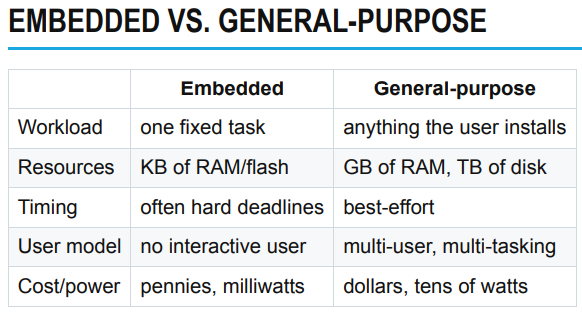
\includegraphics[width=0.5\linewidth]{contents/images/EvsGP.png}
    \caption{Embedded vs General Purpose OS}
\end{figure}

\textbf{\textcolor{red}{Properties: }}
\begin{itemize}
    \item \textbf{Resource Constraints}: It is engineered for \textbf{\textit{minimal overhead}}, operating within strict hardware limits of \textbf{\textit{kilobytes of SRAM (volatile-memory)}} and \textbf{\textit{Flash memory (persistent storage)}} (and operating on milliwatts of power) rather than gigabytes of RAM and massive storage drives.
    \item \textbf{Real-Time Determinism (RTOS)}: Many embedded OSes are Real-Time Operating Systems. This means \textbf{\textit{correctness depends}} not just on the logical output, but \textbf{\textit{on strict temporal deadlines}}. A result computed after its deadline (e.g., sampling a critical sensor every 1 ms) is considered a total system failure, prioritizing deterministic predictability over raw throughput.
    \item \textbf{Flat Memory Architecture}: Embedded OSes \textbf{\textit{frequently utilize a single, flat memory model}}. The startup code, kernel, drivers, and application tasks are all linked into one firmware image sharing a single physical address space, typically without MMU-enforced virtual memory or user-space protection.
    \item \textbf{Static Configuration}: Because the workload is known at compile time, \textbf{\textit{dynamic memory allocation is often replaced by static task counts and fixed buffers}}, and device drivers frequently rely on direct register access rather than heavily abstracted software layers.   
\end{itemize}

\subsection{Monolithic OS Structure}
A monolithic operating system structure is a design where \textbf{\textit{the entire operating system runs as a single, large program in kernel space}}, granting all components direct access to the computer's hardware and memory address space.

\begin{itemize}
    \item \textbf{Kernel Unito}: \textbf{\textit{All core services}}, such as process management, memory management, file systems, and device drivers, \textbf{\textit{live together inside the kernel}}.
    \item \textbf{Shared space}: \textbf{\textit{Every component shares the same memory space}}, meaning parts of the OS can talk to each other directly without message-passing protocols.
    \item  \textbf{Examples}: \textbf{\textit{Linux}} and traditional Unix systems use monolithic or modular-monolithic designs.
\end{itemize}

\begin{figure}[h]
    \centering
    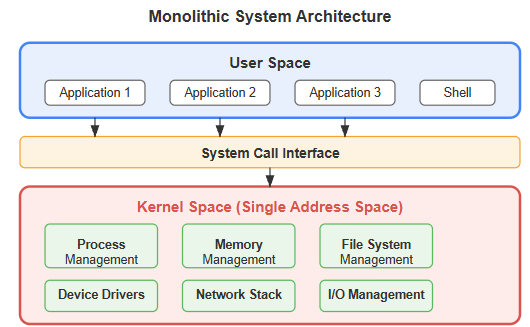
\includegraphics[width=0.8\linewidth]{contents/images/Monolithic.png}
    \caption{Monolithic Operating System Structure}
\end{figure}

\subsection{Microkernel OS Structure}
A microkernel structure is a\textbf{\textit{ minimalist operating system design that keeps only the absolute essential core mechanisms}}, such as low-level address space management, basic thread/process scheduling, and inter-process communication (IPC), in privileged supervisor/kernel mode.

 System services \textbf{\textit{are isolated independent modules, making it easier to update, replace, or unload components}} without rewriting or rebooting the whole system.
Or \textbf{\textit{if a service like a device driver fails, it won’t crash}} the whole system. Each service runs independently, so the core OS remains stable

\textbf{\textcolor{red}{Advantageous:}}
\begin{itemize}
    \item \textbf{Performance}: Because \textbf{\textit{the kernel only contains the essential functions}} required to manage the system, the microkernel design can improve performance. This \textbf{\textit{can make the system faster}} and more efficient.
    \item \textbf{Security}: The microkernel design can improve security by \textbf{\textit{reducing the system's attack surface}} by limiting the functions provided by the kernel. Malicious software may find it more difficult to compromise the system as a result of this.
    \item \textbf{Reliability}: Microkernels are \textbf{\textit{less complex than monolithic kernels}}, which can make them more reliable and less prone to crashes or other issues.
\end{itemize}

\begin{figure}[h]
    \centering
    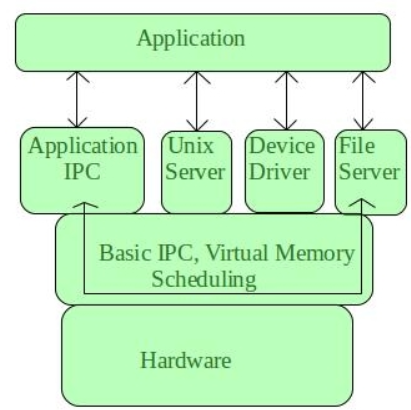
\includegraphics[width=0.5\linewidth]{contents/images/Microkernel.png}
    \caption{Microkernel Operating System Structure}
\end{figure}

\subsection{Flat OS Structure}
A flat structure operating system is an operating system design where \textbf{\textit{components are not separated into rigid hierarchical layers or isolated microkernel spaces, allowing programs to interact closely with or directly access underlying hardware and system services}}.

\textbf{\textcolor{red}{Properties: }}
\begin{itemize}
    \item \textbf{Single Linked Image}: The startup initialization code, the operating system kernel, device drivers, and \textbf{\textit{all application tasks are compiled and linked together into one single executable firmware image stored}} in \textbf{\textcolor{red}{Flash memory}}. There is no process loader dynamically launching separate applications at runtime.
    \item \textbf{Shared Memory}: There is \textbf{\textit{NO virtual-memory translation}} (like an MMU provides in desktop systems). The kernel, all tasks, and device peripherals map \textbf{\textit{directly to the same flat physical memory addresses}}, meaning all components can address the exact same RAM.
    \item\textbf{ No Hardware Isolation}: There is usually \textbf{\textit{no hardware-enforced boundary}} (such as user space versus kernel space) between different tasks.
    \item \textbf{Direct Execution}: \textbf{\textit{Tasks cooperate directly and rapidly through the scheduler and shared memory}}, rather than relying on complex, heavily abstracted inter-process communication.
\end{itemize}       

\textbf{\textcolor{red}{Advantages: }}
\begin{itemize}
    \item \textbf{High Speed}: Offers fast performance because there are fewer operational layers or communication bottlenecks.
    
    \item \textbf{Simple Development}: Easier for programmers to build and manage initially without complex boundary definitions.
\end{itemize}    

\textbf{\textcolor{red}{Disadvantages:}}
\begin{itemize}
    \item \textbf{Vulnerability}: \textbf{\textit{Lacks robust hardware protection and process isolation}}, meaning a single application failure or malicious program can crash the entire system.
    
    \item \textbf{Poor Scalability}: Becomes \textbf{\textit{difficult to maintain, expand}}, or debug as the system grows larger and more complex.
\end{itemize} 

\textbf{\textcolor{red}{Flat Firmware}}
Flat embedded firmware is an architecture where \textbf{\textit{the entire operating system and all applications reside in a single executable image}} operating \textbf{\textit{within one physical address space}}.   

\textbf{Single linked image}: The startup code, kernel, device drivers, and application tasks \textbf{\textit{are all compiled and linked together into one firmware image stored in Flash memory}}.
Tasks cooperate through shared memory and the scheduler.
There is \textbf{no process loader}, \textbf{no virtual-memory translation}, and usually \textbf{no hardware-enforced boundary between tasks}.

\textbf{\textcolor{red}{Flat firmware risks:}}
\begin{itemize}
    \item A simple programming error like \textbf{\textit{a bad pointer in an application task can overwrite}} and corrupt any writable state in the system, \textbf{\textit{including the OS kernel}}.
    
    \item A \textbf{\textit{blocked high-priority task can completely}} halt other important services, effectively \textbf{\textit{freezing the device}}.
\end{itemize}


\subsection{What we will do in the course?}
The \textbf{starting point (scratch-os)}: The course deliberately begins by having you build scratch-os, \textbf{\textit{which utilizes a "flat" firmware architecture}}. This is the simplest possible point on the spectrum. It \textbf{\textit{makes the entire internal pipeline}}, from the initial boot process to task scheduling, \textbf{\textit{completely visible}} and easy to understand.   

\textbf{The Transition (FreeRTOS)}: Later in the course, you will transition to using FreeRTOS. This system is \textbf{\textit{closer to a minimal, microkernel-flavored Real-Time Operating System (RTOS)}}. It features a small dedicated kernel and \textbf{\textit{implements real scheduling policies}}, but it is important to note that, by default, it still does not enforce memory protection between different tasks. 

FreeRTOS provides established, production-ready implementations of the core mechanisms you first build from scratch, such as task creation, priorities, timer-driven scheduling, queues, semaphores, mutexes, and interrupt-to-task communication. The primary reason for this two-step approach is educational: \textbf{\textit{using a high-level RTOS API call becomes much easier to reason about when you already understand the invisible state transitions happening underneath it}}. 

The \textbf{\textcolor{red}{pipeline}} you quoted represents the exact \textbf{\textcolor{red}{sequence of core mechanisms}} you will learn to build manually:

\begin{enumerate}
    \item \textbf{Reset}: Handling the initial hardware state upon powering up.
    
    \item \textbf{Initialise memory}: Setting up the RAM (copying and zeroing data) so C code can safely execute.
    
    \item \textbf{Start application}: Transitioning control to your actual application logic.
    
    \item \textbf{React to events and Schedule tasks}: Handling hardware interrupts and deciding which software task gets CPU time next.
    
    \item \textbf{Synchronise shared resources}: Ensuring that multiple tasks don't corrupt data when accessing the same memory or peripherals.
\end{enumerate}

The main takeaway is that you must build and understand these foundational mechanisms yourself before relying on a production RTOS API. 

\section{Microcontroller (MCU)}
A \textbf{microcontroller (MCU)} \textbf{\textit{integrates onto a single chip the components}} that a desktop computer typically splits across an entire motherboard. It operates as a self-contained system containing:
\begin{itemize}
    \item \textbf{CPU core}: The processor that executes instructions, such as the \textbf{\textit{ARM Cortex-M3}}.
    
    \item \textbf{SRAM}: Volatile \textbf{\textit{working memory}}, which is usually limited to tens of kilobytes.
    
    \item \textbf{Flash}: \textbf{\textit{Non-volatile program storage}} that allows code to run directly from it.
    
    \item \textbf{Peripherals}: \textbf{\textit{Built-in hardware interfaces}} like timers, UART, GPIO, and ADCs.
\end{itemize}

\textbf{\textcolor{red}{Microcontroller VS General-Purpose CPU}}
\begin{itemize}
    \item \textbf{Integration}: \textbf{\textit{A general-purpose desktop CPU is just the processing core}}; \textbf{\textit{it must use external buses}} to reach separate chips for RAM, storage, and I/O. An \textbf{\textit{MCU has all of these elements built}} directly into the \textbf{\textit{same chip}}.   
    
    \item \textbf{Memory Management}: A desktop CPU utilizes a Memory Management Unit \textbf{\textit{(MMU) to give}} every running process its own \textbf{\textit{isolated virtual address space}}. \textbf{\textit{An MCU}} relies on one flat physical address map shared by the code, data, and every peripheral register, meaning it \textbf{\textit{has no virtual memory and no MMU}} (a Cortex-M relies at most on an optional Memory Protection Unit).   
    
    \item \textbf{Hardware Interaction}: On an MCU, "the hardware" is simply memory that you write to directly. \textbf{\textit{Unlike general-purpose systems, there is no abstraction or driver layer}} sitting between your code and a device register.
\end{itemize}

\section{From Hardware To Software}
\subsection{QEMU (Virtual Hardware)}
\begin{itemize}
    \item Cos'è: QEMU è un emulatore software in esecuzione sul tuo computer (l'host) che simula fisicamente il comportamento di una specifica scheda a microcontrollore ARM (il target).   
    
    \item A cosa serve: Invece di costringerti a comprare e cablare una vera scheda elettronica, QEMU ti fornisce un ambiente identico e riproducibile (la macchina mps2-an385) su cui caricare e testare il tuo firmware. È la "finta" CPU ARM Cortex-M3 su cui girerà tutto il tuo codice. 
\end{itemize}

\subsection{Scratch-OS}
\begin{itemize}
    \item Cos'è: È un piccolissimo sistema operativo flat (piatto) che costruirete voi stessi da zero durante la prima parte del corso.  
    
    \item A cosa serve: Serve a svelare tutta la "magia invisibile" che c'è dietro ai sistemi operativi. L'obiettivo di scratch-os è farti scrivere a mano tutti quei meccanismi fondamentali che un OS normalmente nasconde: gestire il reset, inizializzare la RAM, reagire agli interrupt hardware e creare un basilare scheduler per far girare più task. 
\end{itemize}

\subsection{FreeRTOS}
\begin{itemize}
    \item Cos'è: È un vero e proprio Real-Time Operating System (RTOS) utilizzato nell'industria, basato su un'architettura più vicina a un microkernel.   
    
    \item A cosa serve: Una volta capito come si costruisce un OS (grazie a scratch-os), nella seconda parte del corso butterete via il vostro kernel manuale e inizierete a usare FreeRTOS. Questo vi permetterà di usare API standard e professionali per creare task, gestire priorità, code e semafori. Usare FreeRTOS diventerà facilissimo proprio perché, avendo costruito prima scratch-os, saprai esattamente cosa succede "sotto il cofano" a livello di registri e memoria. 
\end{itemize}

\subsection{mps2-an385}
mps2-an385 è il modello esatto di scheda che QEMU sta simulando. La scheda definisce la "mappa" del sistema: dice a QEMU che la memoria Flash parte dall'indirizzo 0x00000000, la SRAM da 0x20000000 e che ci sono specifiche periferiche (come l'output seriale) a determinati indirizzi.

The mps2-an385 machine board structure represents an ARM V2M-MPS2 (Cortex-M Prototyping System 2) motherboard configured via Application Note AN385. In this implementation, the ARM Cortex-M3 processor core and its primary system design kit (CMSDK) peripherals are synthesized within the board's onboard FPGA.

\subsection{ARM Cortex-M3}
L'ARM Cortex-M3 è un core di processore RISC a 32 bit progettato da ARM Holdings specificamente per applicazioni embedded a basso costo, bassa potenza e ad alte prestazioni.
\begin{figure}
    \centering
    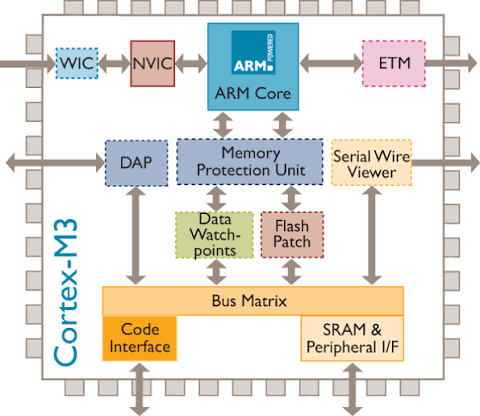
\includegraphics[width=0.5\linewidth]{contents/images/Cortex_M3.png}
    \caption{ARM Cortex-M3 microcontroller}
\end{figure}









\section{Machine Model}
\subsection{Cortex-M3 at Reset step}
When the \textbf{Cortex-M3} processor \textbf{\textit{is powered on}} or reset, it does not look for or discover an operating system. 

The sequence \textbf{\textit{involves two pointers}} (32-bit values) and it happens \textbf{\textit{entirely in hardware}} (directly readed from the vector table located in the Flash, \textbf{\textit{typically address 0x00000000}} is where the \textbf{vector table} is stored.) \textbf{\textit{before}} a single line of \textbf{\textit{your software is executed}}.

Those 2 lines provide the absolute minimum orientation it needs to function: a place to temporarily store data (RAM) and a place to start reading instructions (Flash).

\begin{enumerate}
    \item \textbf{Main Stack Pointer}: Tells the \textbf{\textcolor{red}{CPU's internal Stack Pointer register}} exactly where the top of the stack is located in the \textbf{\textit{SRAM (volatile memory)}}.
    \item \textbf{Reset Handler Address}: provides the initial value for the \textbf{\textcolor{red}{Program Counter}}, pointing it directly to a specific address in the \textbf{\textit{Flash memory (non-volatile memory)}} where your boot code lives.
\end{enumerate}

Once these two pointers are read, \textbf{\textit{the automated hardware boot phase is complete}}. The hardware hands over control to your software (the Reset\_Handler), which now relies on the newly established stack to prepare the C runtime environment and \textbf{\textcolor{red}{ultimately call your main() function}}.

\textbf{\textcolor{red}{CPU working on registers}}
The CPU operates on values held in registers. Memory is accessed explicitly
with load and store instructions.

\begin{figure}[h]
    \centering
    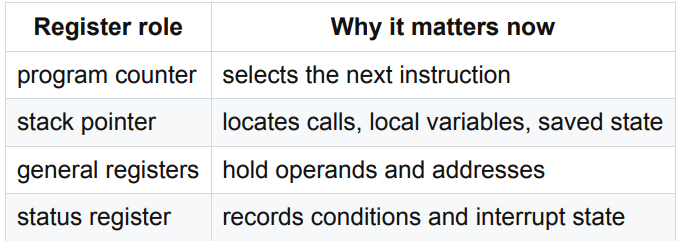
\includegraphics[width=0.8\linewidth]{contents/images/registers.png}
    \caption{Most used registers of ARM Cortex-M3}
\end{figure}

\subsection{Components}
Flash vs SRAM (Static RAM) roles:
\begin{itemize}
    \item \textbf{Flash Memory}: This is \textbf{\textit{non-volatile storage}}. It permanently stores the vector table, \textbf{\textit{the executable instructions}} (\textcolor{red}{.text section}), read-only \textbf{\textit{constants}} (\textcolor{red}{.rodata}), and the \textbf{\textit{initial byte values}} required for your initialized variables (\textcolor{red}{the initial .data image}).  
    
    \item \textbf{SRAM (Static RAM)}: This is fast, volatile working memory. It holds the actively used \textbf{\textit{initialized variables}} (\textcolor{red}{.data}), the \textbf{\textit{zero-initialized variables}} (\textcolor{red}{.bss}), the \textbf{\textit{heap area, and the stack}}.   
    
    \item \textbf{The Startup Requirement}: Because SRAM forgets everything when the system restarts, your custom \textbf{\textit{startup code must physically copy the initial values}} for the \textcolor{red}{.data} section \textbf{\textit{from Flash into SRAM}}, and explicitly clear the \textcolor{red}{.bss} section to zero before standard C code can safely execute.
\end{itemize}

\begin{figure}[h]
    \centering
    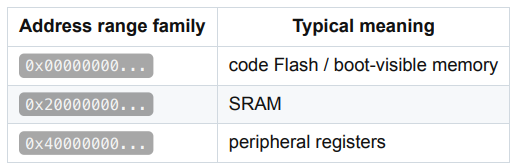
\includegraphics[width=0.8\linewidth]{contents/images/Memory_Addresses.png}
    \caption{Memory addresses begin}
\end{figure}

\textbf{Load/Store Architecture}: The Cortex-M3 executes a load/store instruction set. \textbf{\textit{To process data}}, a \textbf{\textcolor{red}{load instruction}} must bring the value from a specific memory address into a register, and a \textbf{\textcolor{red}{store instruction}} must \textbf{\textit{write}} the computed result \textbf{\textit{back to memory}}.

\begin{figure}[h]
    \centering
    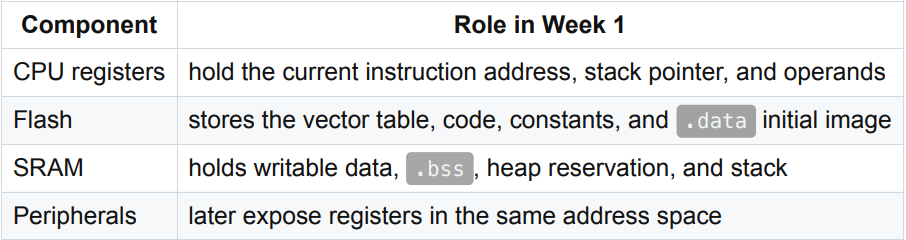
\includegraphics[width=0.85\linewidth]{contents/images/devices.png}
    \caption{Roles of each component inside the Cortex-M3}
\end{figure}












